\section{Complexity Lower Bounds}
\begin{definition}
    A function $f(n)$ is called a \textit{complexity lower bound}
    for a computational problem $L$
    in a given class $M$ of models of computation
    if for any algorithm from $M$ which solves $L$ with complexity $T(n)$ the following relation holds:
    $$T(n) = \Omega(f(n))$$
\end{definition}

\textbf{Key Points}
\begin{itemize}
    \item Very few natural problems have proven lower bounds in the class of all Turing machines because these models are powerful.
    \item An example is the quadratic lower bound for the problem of recognizing palindromes
        (in the class of one-tape, one-head Turing machines).
    \item Clearly it should be easier to prove lower bounds for narrower classes $M$.
\end{itemize}

\subsection{Decision Trees}
\textbf{A Lower Bound for Comparison Sorting}\\
We can arrive at a lower bound for comparison based for sorting using decision trees.

\begin{itemize}
    \item \textbf{Input}:
        A finite set $X = \{x_1,\dots x_n\}$ and
        a binary relation $\leq$ on $X$ where we have reflexivity, anti-symmetry, and transitivity.
    \item \textbf{Output}:
        A list containing all the elements of $X$ such that elements are in order.
        $$x_i \leq x_j \leq \dots$$
\end{itemize}

Consider sorting three items $(a,b,c)$,
we can derive a decision tree.
At each node of the tree we compute one binary relation
the left child will represent the result of the computation being true
conversely the right child will mean the computation result was false.
\begin{center}
    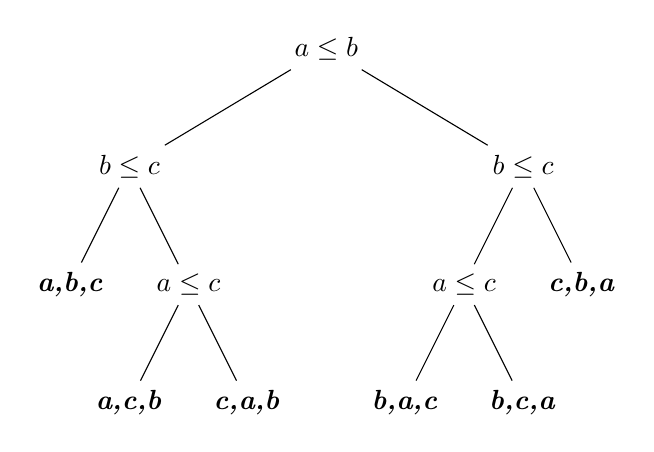
\begin{tikzpicture}[level distance=1.5cm,
  level 1/.style={sibling distance=5cm},
  level 2/.style={sibling distance=1.5cm},
  level 3/.style={sibling distance=1.5cm}]
  \node {$a \leq b$}
    child {node {$b \leq c$}
        child {node {\textbf{\textit{a,b,c}}}}
        child {node {$a \leq c$} {
          child {node {\textbf{\textit{a,c,b}}}}
          child {node {\textbf{\textit{c,a,b}}}}
      }}
    }
    child {node {$b \leq c$}
        child {node {$a \leq c$} {
          child {node {\textbf{\textit{b,a,c}}}}
          child {node {\textbf{\textit{b,c,a}}}}
      }}
          child {node {\textbf{\textit{c,b,a}}}}
    };
\end{tikzpicture}
\end{center}

Observe that the height or depth of the tree represents the amount of computations which must be performed.
Furthermore the height of the tree is not the same for every leaf node (computation result).\\

This is because we can prune some branches due to the transitive property of $\leq$,
given $a \leq b$ and $b \leq c$ we also know that $a \leq c$ is true.
Thus we do not need to compute $a \leq c$.
Conversely given $a \leq b$ and $c \leq b$ we \textbf{do not know}
anything about $a \leq c$.
This is another computation we need to perform to have a correct ordering.\\

Obviously this tree is correct for $n = 3$, so we can say
the complexity lower bound for $n = 3$ is 3 computational steps.
This is because equipped with only comparison we can only go in one
of two directions after each computation (true or false),
and we must be able to produce all six possible orderings.

Well for a three item set $(a,b,c)$ there exists precisely $!3 = 6$ orderings,
or more generally there exists for an $n$ item set $!n$ orderings.
Because this model of computation is binary decision trees,
we can only have $2^x$ leafs (or results) given $x$ computations,
however we need $!n$ leafs therefore, given this information
we can show that comparison sorting has $\Omega(n log_2 n)$.
\begin{align*}
    2^x &\geq !n \\
    x &\geq \log_2(!n) \\
    \log_2(!n) &= \log_2n + \log_2(n − 1) + \dots + \log_2(2)\\
               &= \Omega(n\log_2n)
\end{align*}

\subsection{Algebraic Computation Trees}
\textbf{Algebraic Computation Trees: Examples}\\
We can expand the decision tree model to something more powerful.
Consider the problem of finding if a point is inside the unit circle:
\begin{itemize}
    \item \textbf{Input}:A point $(x,y) \in \mathbb{R}^2$
    \item \textbf{Output}: Yes iff $x^2 + y^2 \leq 1$
\end{itemize}

\begin{center}
    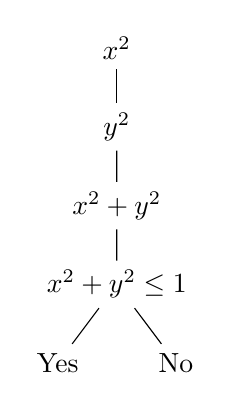
\begin{tikzpicture}[level distance=1cm,
  level 1/.style={sibling distance=2cm},
  level 2/.style={sibling distance=1.5cm},
  level 3/.style={sibling distance=1.5cm},
  level 4/.style={sibling distance=1.5cm},
  level 5/.style={sibling distance=1.5cm}]
  \node {$x^2$}
        child {node {$y^2$}
        child {node {$x^2 + y^2$}
        child {node {$x^2 + y^2 \leq 1$}
            child {node {Yes}}
            child {node {No}}
            }}
        };
\end{tikzpicture}
\end{center}

The complexity of this algorithm (the height of the tree) is 4, i.e., a constant.
This is quite natural since we assume that the size of the input is a constant.
To further generalise our algebraic computation trees,
we will say that every node, except leaves, have three children.
The children correspond to the computation being $(= 0), (< 0), (> 0)$.

\begin{center}
    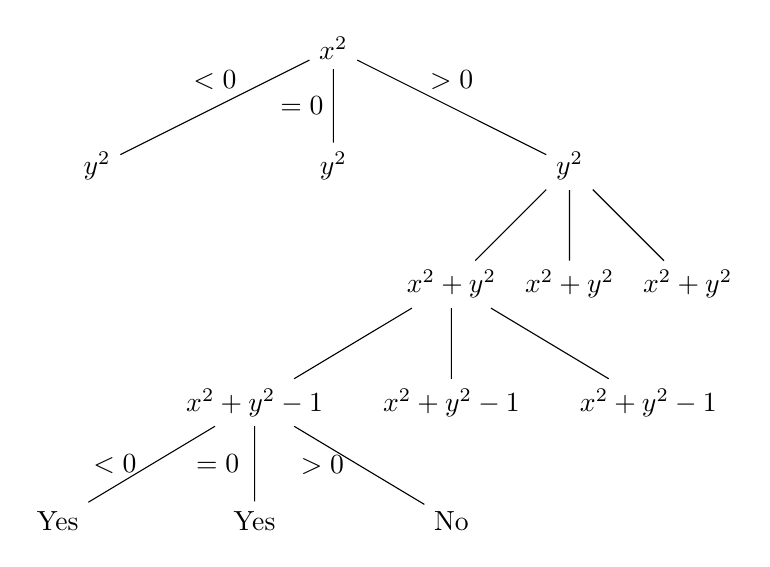
\begin{tikzpicture}[level distance=1.5cm,
  level 1/.style={sibling distance=3cm},
  level 2/.style={sibling distance=1.5cm},
  level 3/.style={sibling distance=2.5cm},
  level 4/.style={sibling distance=2.5cm}]
    \node {$x^2$}
            child {node {$y^2$} edge from parent node[left,above=3pt] {$< 0$}
            }
            child {node {$y^2$} edge from parent node[left] {$= 0$}
            }
            child {node {$y^2$}
                child { node {$x^2 + y^2$} 
                    child { node {$x^2 + y^2 - 1$} 
                        child { node {Yes} edge from parent node[left=2pt] {$< 0$}}
                        child { node {Yes} edge from parent node[left=2pt] {$= 0$}}
                        child { node {No}  edge from parent node[left=2pt] {$> 0$}}
                    }
                    child { node {$x^2 + y^2 - 1$} }
                    child { node {$x^2 + y^2 - 1$} }
                }
                child { node {$x^2 + y^2$} }
                child { node {$x^2 + y^2$} }
            edge from parent node[left,above=3pt] {$> 0$} }
       ;
\end{tikzpicture}
\end{center}

In the example above for the sake of brevity we don't show all the different branches,
simply because we never make any changes to our computation dependent on the result;
that is until the very end where we use it for our yes or no result.
This tree, were it completed, would have $3^4 = 81$ nodes,
much more than our previous tree.
However observe that the height remains unchanged at four,
thus the complexity is the same.\\

One can generalise this example from membership of the unit circle to membership
of the $n$ dimensional unit ball. Simply calculate
$$1 \leq \sum_{i=1}^{n} x_i^2$$
You calculate $x_i^2$ for the $i$-th dimension and add it to the running total;
this takes $2n$ steps.
In case $n = 2$ we get complexity four as our computation tree showed.\\

\textbf{Algebraic Computation Trees: Definition}
\begin{definition}
    A subset $S \subset R^n$ is called \textit{(basic) semi-algebraic} if it is defined by
    $$\{P_1(x_1,\dots x_n) = 0,\dots P_n\}
    \cup
    \{Q_1(x_1,\dots x_n) > 0,\dots Q_m\}$$
    where $P_i$ and $Q_j$ are polynomials in $n$ variables
    i.e., S is a set of all solutions of a system of equations and strict inequalities.
\end{definition}

Algebraic computation tree $T$ in variables $x_1,\dots x_n$
is a tree with the root $v_0$ such that to every vertex $v$ (except leaves)
is an arithmetic operation (addition, subtraction or multiplication) 
and a polynomial $f_v$ is attached.\\

For example $f_3 = f_1 + f_2$ where $f_3$ is the new polynomial;
more precisely in our previous example membership of the unit circle
we have
$$f_1 = x^2 \quad f_2 = y^2 \quad f_3 = x^2 + y^2$$
$$f_4 = f_3 - 1 = x^2 + y^2 - 1$$

\textbf{Semi-Algebraic Sets and Algebraic Computation Trees}\\
Let $v_0, v_1,\dots, v_\omega$ be the sequence of vertices
along the (unique) branch leading from the root $v_0$ to $v_\omega$.
An arithmetic operation at $v_i$ is performed on a pair from
$$\{x_1,\dots x_n\} \cup \{f_0\dots f_{i - 1}\}$$
and the result is at $f_i$.
Note that every $v$ has exactly three children.\\

Let $*_i \in \{>0,=0,<0\}$ for $0 \leq i < \omega$ be the sign of $f_{v_i}$,
One can assign the semi-algebraic set $U_\omega$ to $v_\omega$
$$U_\omega = \{f_0*_00,f_1*_10\dots f_{\omega - 1} *_{\omega - 1}0\}$$

To each leaf $\omega$ of $T$ an output Yes or No is assigned.
We call $U_\omega$ an accepting set if the leaf $\omega$ has the output Yes assigned.
We say that T tests the membership to the union of all accepting sets.\\

To illustrate this relation between
semi-algebraic sets and algebraic computation trees,
consider our unit circle example computations which works as follows.
A specific point $x \in \mathbb{R}^n$ is taken as an input.
Then the value $f_{v_0}(x)$ is computed and the sign of this value is determined.
According to the sign, the algorithm goes to the corresponding child $v_1$ of $v_0$.
If the process eventually arrives to a Yes-vertex, then $x$ belongs to an accepting set,
and, therefore, to the union of all accepting sets.\\

\textbf{Distinctness Problem: Upper Bound}
\begin{itemize}
    \item \textbf{Input}: $(x_0, x_1,\dots x_n) \in \mathbb{R}^n$
    \item \textbf{Output}: Yes iff $\forall\ i,j$ where $0 \leq i,j \leq n, i \neq j$ we have $x_i \neq x_j$
\end{itemize}
An immediate solution for this problem is to sort the numbers $(x_0, x_1,\dots x_n)$
then compare pairwise neighbours for equivalence;
this has complexity $O(nlogn)$.
It is clear that this algorithm can be represented in a form of algebraic computation tree
of the height $O(nlogn)$ (compare with sorting).
We are going to develop a general method for proving lower complexity bounds for algebraic computation trees,
and will apply this method to prove the $\Omega(nlogn)$ lower bound for Distinctness.\\

\textbf{Connected components of Semi-Algebraic Sets}\\
Informally,
a finite union $W$ of semialgebraic sets is called connected
if for every $x, y \in W$ there is a “continuous” curve in $W$ containing both $x$ and $y$.
A formal definition can be found in textbooks on topology.

\begin{definition}
    Any maximal (with respect to the set-theoretical inclusion) connected subset of W is called connected component of W.
\end{definition}

\begin{theorem}
    Every finite union $W$ of semialgebraic sets
    can be uniquely represented as a union of a finite number of its connected components
    (which are finite unions of semialgebraic sets):
    $$W = \bigcup\limits_{1\leq i \leq k} W_i$$
\end{theorem}

\begin{example}
    Consider these examples
    \begin{enumerate}
        \item The union of open intervals $W = (0, 1) \cup (2, 3) \subset R$ is \textbf{not connected}.
            Intervals $(0, 1)$ and $(2, 3)$ are connected components of W .
        \item The union $W = (0, 1) \cup (1, 2)$ is \textbf{not connected} with $(0, 1),\ (1, 2)$ being $W$’s connected components.
        \item The union $W = (0, 1) \cup 1 \cup (1, 2) = (0, 2)$ \textbf{is connected} and is its own unique connected component.
        \item The semialgebraic set $W = \{X \neq Y \} \in R^2$
            (which also can be written in the form $W = \{X^2 − 2XY + Y^2 > 0\}$)
            is \textbf{not connected} and has two connected components: $\{X − Y > 0\}$ and $\{Y − X > 0\}$.
    \end{enumerate}
\end{example}

\begin{theorem}
    Projection of a connected set $W \subset \mathbb{R}^{n+m}$
    on a coordinate subspace $\mathbb{R}^n$ is also connected.
\end{theorem}

\textbf{Lower Bound for Membership to a Semi-Algebraic Set: Decision Computation Trees}

\begin{definition}
    Let the union $\Sigma$ of all accepting sets
    of an algebraic computation tree $T$
    have $\nu(\Sigma)$ connected components.
\end{definition}

\begin{theorem}
    The height $k$ of a \textbf{decision computation tree} $T$,
    i.e. the complexity of testing membership to $\Sigma$,
    is $\Omega(\log\nu(\Sigma))$.
\end{theorem}

\begin{proof}
    Observe that any non-empty accepting set $W$ of $T$
    is a set of all points in $\mathbb{R}^n$ satisfying a system of linear equations and strict linear inequalities,
    and is, therefore, a convex polyhedron in $\mathbb{R}^n$.  It follows that
    $$\nu(W) = 1$$
    Since there is at most $3^k$ leaves in $T$, we get
    \begin{align*}
                3^k &\geq \nu(\Sigma) \\
                  k &\geq c\log \nu(\Sigma)
    \end{align*}
    Taking the binary logarithm in both parts,
    we obtain an inequality for a constant $c > 0$,
    hence we have
    $$\Omega(\log\nu(\Sigma))$$
\end{proof}

\textbf{Thom-Milnor’s bound}\\
\begin{theorem}
    \textit{(R. Thom, J. Milnor)}
    Let a semialgebraic set $W$ be defined by a system of
    equations and strict inequalities with polynomials of degree at most $d$ in $n$ variables,
    having $m$ inequalities.
    Then the number of all connected components of $W$ does not exceed
    $$((m + 1)d)^{cn}$$
    for a constant $c > 0$.
    The known proofs of Thom-Milnor’s bound use complex arguments from differential and algebraic topology,
    we are not considering them.
\end{theorem}

\begin{theorem}
    Let $W$ be a semialgebraic set satisfying the conditions of the theorem.
    Then the number of the connected components of a projection of $W$ on any coordinate subspace does not exceed
    $$((m + 1)d)^{cn}$$
    for a constant $c > 0$.
\end{theorem}

\begin{theorem}
    \textit{(M. Ben-Or)}
    Let the union $\Sigma$ of all accepting sets of an \textbf{algebraic computation tree} $T$
    have $\nu(\Sigma)$ connected components.
    Then the height $k$ of $T$ (the complexity of testing membership to $\Sigma$) is
    $$\Omega(\log(\nu(\Sigma)) − n)$$
\end{theorem}

\textbf{Distinctness problem: lower bound}\\
\begin{theorem}
    Distinctness problem has a complexity lower bound $\Sigma(n \log n)$.
\end{theorem}
\begin{proof}
    The union $\Sigma$ of all accepting sets in this problem
    is the complement to the union of hyperplanes defined by
    all possible linear equations of the kind
    $$X_i = X_j$$
    where $i \neq j$,
    in other words,
    at a point $x = (x_1, \dots x_n) \in \Sigma$ all coordinates are pairwise distinct
    (briefly consider the to $W = \{X \neq Y \} \in R^2$).
    Herewith, the coordinates of $x$ are somehow ordered:
    $$x_{i_1} < \dots < x_{i_n}$$
    It is easy to see that,
    at each point of a connected component $\Sigma_i$ of $\Sigma$
    the order of the coordinates is the same.
    Indeed, suppose this is wrong, and for two points
    $$y = (y_1, \dots , y_n)\quad z = (z_1, \dots , z_n)$$
    we have $y_l < y_m$,
    but $z_l > z_m$.
    By the definition of connectedness,
    there is a continuous curve in $\Sigma_i$ connecting $y$ and $z$.
    Since the values of coordinates change continuously along the curve,
    there should be a point $w = (w_1, \dots , w_n)$ on the curve such that $w_l = w_m$.
    Thus, $w \in {X_l = X_m}$,
    that is, $w$ belongs to the complement of $\Sigma$, which is a contradiction.\\

    We have proved that the number of connected components of $\Sigma$
    is not less than the number $n!$ of all permutations of $n$ coordinates (in fact these numbers coincide).
    According to the Thom-Milnor’s theorem, we get a lower bound
    \begin{align*}
        &\Omega(\log(n!)) \\
        &\Omega(n \log n)
    \end{align*}
\end{proof}
